% =====================================================================
% DeepSpine: article in IEEE conference format (English version)
% Course template: US letter, two columns, Times, "TABLE I" above tables
% and "Fig. 1" below figures, at most three heading levels (III. / A. / 1)).
% Build: pdflatex -> bibtex -> pdflatex -> pdflatex
% (on Overleaf, upload the folder and compile main.tex).
% =====================================================================
\documentclass[conference,letterpaper]{IEEEtran}
\usepackage[utf8]{inputenc}
\usepackage[T1]{fontenc}
\usepackage{amsmath}
% Las tablas y figuras nunca aparecen antes del punto del texto donde se escriben
\usepackage{flafter}
\usepackage{graphicx,booktabs,array,xcolor}
\usepackage{url}
\def\UrlBreaks{\do\_\do\-\do/\do.}
\usepackage{tikz,pgfplots}
\usetikzlibrary{positioning,arrows.meta}
\pgfplotsset{compat=1.16}
\graphicspath{{figures/}}

\begin{document}

\title{DeepSpine: Classification of Lumbar Intervertebral Discs in Sagittal T2-Weighted MRI}

\author{\IEEEauthorblockN{Jhon Jairo Perdomo Perdomo, Julián Andrés Silva Morales, Juan Manuel Tengonó Lasso}
\IEEEauthorblockA{\textit{Software Engineering Program, Faculty of Engineering, Universidad Surcolombiana}\\
\textit{Neiva, Colombia}\\
{\small\ttfamily u20221203988@usco.edu.co}\\
{\small\ttfamily u20221203367@usco.edu.co}\\
{\small\ttfamily u20202193898@usco.edu.co}}}

\maketitle

\begin{abstract}
Diagnosing lumbar intervertebral disc pathology on magnetic resonance imaging (MRI) is a manual task that varies between observers. This work presents DeepSpine, an end-to-end pipeline that classifies lumbar discs on sagittal T2-weighted slices into three classes: Normal, Disc Degeneration and Protrusion. Starting from a public dataset of 515 patients, a dataset of 5,123 per-disc regions of interest (ROIs) from 399 patients was built through series cleaning, disc detection with YOLOv8n, model-assisted pre-labeling with human review of every ROI, and a 70/15/15 patient-level split; data augmentation, applied within each partition, brought the set to 35,007 images. Four models were compared under the same split and the same metrics: fine-tuned YOLOv8s-cls and ResNet-50, and an SVM and a Random Forest trained on features from the fine-tuned ResNet-50. On the 768 original test ROIs, ResNet-50 achieved the highest accuracy (88.9\%; 95\% CI: 86.5--91.0) and the highest macro F1 (0.769), although the differences among the four models fall within the margin of error. All models recognize Protrusion well (recall $\geq 0.94$) and struggle with Degeneration (recall of 0.40 to 0.50). Classical classifiers match the networks only when they operate on task-adapted features. The limit appears to lie in the data (labels without a radiologist, few Degeneration cases and a strong vertebral-level bias) rather than in the architecture.
\end{abstract}

\begin{IEEEkeywords}
magnetic resonance imaging, lumbar intervertebral disc, image classification, deep learning, patient-level split, ResNet-50, YOLOv8.
\end{IEEEkeywords}

\section{Introduction}
% I. Introduction
Low back pain is the leading cause of years lived with disability worldwide: in 2020 it affected about 619 million people, and it is projected to reach 843 million cases by 2050 \cite{gbd2023}. Magnetic resonance imaging (MRI) is the reference imaging test for the intervertebral disc. On sagittal T2-weighted slices, loss of disc signal and height indicates degeneration, according to the Pfirrmann scale \cite{pfirrmann2001}, and the extension of disc material beyond its margins defines bulges and herniations, according to the consensus nomenclature \cite{fardon2014}.

Reading these studies is manual, time-consuming and dependent on the reader's experience. Even with a standardized nomenclature, inter-radiologist agreement on disc contour is only fair to moderate \cite{arana2011}. A support system that automatically classifies the state of each disc could shorten reading time and make criteria more consistent. Computer vision has already been applied to this task with good results \cite{sari2025,tan2024,sayed2025scirep,wang2025}, but many figures come from small test sets, from binary tasks or from splits not declared at the patient level, and they drop when evaluated on external data \cite{yi2023,nigru2024}. When the same patient contributes images to both training and test sets, the model may recognize the patient instead of the pathology, inflating the metrics \cite{brunekreef2024,rumala2023}.

This work presents DeepSpine, an end-to-end pipeline to classify lumbar discs (L1-L2 to L5-S1) on sagittal T2-weighted slices of the \emph{Lumbar Spine MRI Dataset} \cite{sudirman2019}. The initial project proposal defined four classes (Normal, Degeneration, Bulge and Herniation) and three research questions:
\begin{enumerate}
  \item[Q1.] \textbf{Exploratory analysis:} how are the cases of each class distributed in the dataset, and which visual differences (brightness, shape or size) distinguish a healthy disc from a pathological one?
  \item[Q2.] \textbf{Classical versus deep learning:} can simpler and faster classical algorithms (SVM or Random Forest) achieve a reliable diagnosis from image features, or is a deep neural network required?
  \item[Q3.] \textbf{Deep learning:} which convolutional neural network architecture achieves the highest accuracy (with a target above 90\%) and the lowest false-negative rate?
\end{enumerate}
During dataset construction, Herniation and Bulge proved inseparable on the sagittal plane and were merged into a single class, Protrusion (Section~\ref{sec:annotation}); the three questions are therefore answered over three classes.

The contributions are threefold: (i) a dataset of 5,123 ROIs from 399 patients, built with a traceable process that is reproducible from the public data and that declares its errors and limitations; (ii) a comparison of four models from different families (YOLOv8s-cls, ResNet-50, SVM and Random Forest) under the same patient-level split, the same metrics and evaluation on original images; and (iii) an analysis of class imbalance and vertebral-level bias that puts the achieved accuracy into perspective. Section~\ref{sec:related} reviews prior work; Section~\ref{sec:methodology} describes the dataset construction, the problem formulation and the models; Section~\ref{sec:results} presents and discusses the results; and Section~\ref{sec:conclusions} answers the research questions and outlines limitations and future work.


\section{Related Work}
\label{sec:related}
% II. Related Work
\subsection{Lumbar MRI Datasets}
The \emph{Lumbar Spine MRI Dataset} contains studies from 515 patients with symptomatic low back pain \cite{sudirman2019}. On the same corpus, Natalia \emph{et al.} selected the 515 mid-sagittal T2 slices and predicted the Pfirrmann grade with a mean accuracy of 88.1\% \cite{natalia2024}, and Masood \emph{et al.} released 1,545 radiologist-validated Pfirrmann grades for L3-L4, L4-L5 and L5-S1 \cite{masood2026}. Beyond this corpus, SPIDER provides 447 sagittal T1 and T2 series from 218 patients at four hospitals, annotated iteratively \cite{vandergraaf2024}, and LumbarDISC gathers 2,697 patients from eight institutions in six countries, annotated by expert radiologists \cite{richards2026}. Multicenter, expert-annotated datasets are the reference for validating models, but Sudirman's dataset remains one of the few that allow working with individual discs within an academic timeframe.

\subsection{Disc Classification with Deep Learning}
The YOLO family is the most common in the reviewed work. Liawrungrueang \emph{et al.} detected and graded degeneration with YOLOv5 on 1,000 sagittal T2 images from 515 patients, with accuracy above 95\% \cite{liawrungrueang2023}; Prisilla \emph{et al.} compared YOLOv5x, YOLOv6 and YOLOv7 for herniation detection with radiologist labels \cite{prisilla2023}; Wang \emph{et al.} graded degeneration and herniation with a modified YOLO on sagittal and axial T2 images, with 420 internal and 52 external patients \cite{wang2025}. Sayed \emph{et al.} used YOLOv8 to detect discs and crop one ROI per disc on sagittal slices (mAP50 of 99.4\% for the disc) \cite{sayed2025scirep}, and a cascade of a detector and a CNN to identify discs and detect herniation on axial and sagittal slices \cite{sayed2025imu}. With residual networks, Tan \emph{et al.} combined ResNet-50 and YOLOv2 to classify healthy and herniated discs, although with only 32 patients (160 discs) \cite{tan2024}, and Al-kubaisi and Khamiss applied transfer learning to the same four classes as this project in 181 patients, mostly on axial slices \cite{alkubaisi2022}. In computed tomography, bulge and protrusion were the most confused pair of classes \cite{gao2025}.

\subsection{Deep Features with Classical Classifiers}
On Sudirman's corpus, Sar{\i} and Atasoy extracted features with ResNet-50, selected them with grey wolf optimization (GWO) and classified them with an SVM, reaching 99.42\% on a binary task with T1 slices and five-fold cross-validation, without stating whether the split was patient-level \cite{sari2025}. Khoiwal and McMillan showed that linear classifiers on frozen embeddings match models trained from scratch on retinal, mammography, dermoscopy and chest images \cite{khoiwal2024}. On tabular spine data (bone angles), the best classifier was a SMOTE-RFE-XGBoost model \cite{zhang2023}.

\subsection{Research Gap}
The highest results in the literature (97--99\%) correspond to binary tasks or small test sets, and internal figures drop under external validation: in one study, the sagittal F1 fell from 0.971 to 0.768 and 0.787 at two external centers \cite{yi2023}. Few studies on Sudirman's corpus declare a patient-level split, report per-class metrics under the real imbalance or analyze biases such as the vertebral level. This work addresses that gap: it compares four model families under the same patient-level split, evaluates on original images and reports per-class and per-level metrics.


\section{Methodology}
\label{sec:methodology}
% =====================================================================
% III. Methodology: dataset construction (subsections A to G).
% Fragment without \section; followed by sections/methodology_models.tex (H to J).
% Heading levels: \section -> III.  \subsection -> A.  \subsubsection -> 1)
% =====================================================================
\providecommand{\arch}[1]{\path{#1}}

This section describes, in order, how the original public dataset was turned into the 35,007 region-of-interest (ROI) images used to train and compare the four models (Sections~\ref{sec:models} and \ref{sec:protocol}). Fig.~\ref{fig:pipeline} summarizes the pipeline and the number of items at each stage. All figures come from files versioned in the project repository.

% ---------------------------------------------------------------------
\subsection{Data Source}
\label{sec:origin}
The \emph{Lumbar Spine MRI Dataset} (Mendeley Data) \cite{sudirman2019} was used. It contains studies from 515 patients with symptomatic low back pain and 48,345 MRI slices, and it has already been used in previous work on disc herniation classification \cite{sari2025} and on Pfirrmann grading of degeneration \cite{natalia2024}. The studies were acquired on a single scanner, a 1.5~T Siemens MAGNETOM Essenza, and are distributed as DICOM files with the \arch{.IMA} extension, in one folder per patient. Folders are numbered 0001 to 0575; the 60 missing numbers are already missing at the source. Slices have a pixel size of 0.729~mm, a thickness of 4~mm and a center-to-center spacing of 4.8~mm. The \texttt{.IMA} files keep their DICOM metadata, but the \texttt{PatientID} field is empty throughout the corpus and the source only keeps study and series identifiers. Therefore, in this work each folder is treated as one patient: the 515 folders correspond to the 515 patients, and every mention of ``patient'', including the patient-level split, refers to the folder.

Of the 515 patients, 414 kept usable slices after cleaning (Section~\ref{sec:cleaning}) and 399 after the ROI quality exclusions (Section~\ref{sec:roi}). Each of the 414 folders corresponds to a different \texttt{StudyInstanceUID} and no \texttt{StudyTime} is repeated; there is no evidence of duplicated patients, although, with the identifier empty, this cannot be fully ruled out.

\begin{figure}[!htb]
\centering
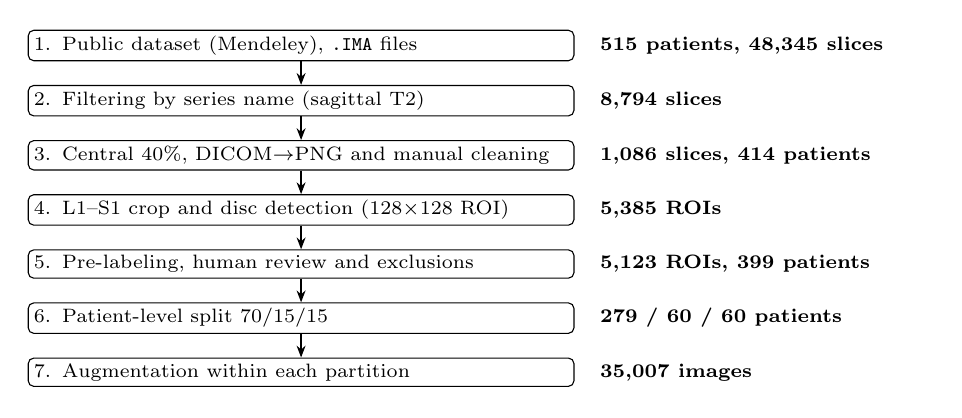
\begin{tikzpicture}[
  box/.style={draw, rounded corners=2pt, align=left, text width=0.56\columnwidth, inner sep=2pt, font=\scriptsize},
  num/.style={align=left, text width=0.34\columnwidth, font=\scriptsize\bfseries},
  arrow/.style={-{Stealth[length=1.5mm]}, thick},
  node distance=3mm]
  \node[box] (a) {1. Public dataset (Mendeley), \texttt{.IMA} files};
  \node[num, right=2mm of a] {515 patients, 48,345 slices};
  \node[box, below=of a] (b) {2. Filtering by series name (sagittal T2)};
  \node[num, right=2mm of b] {8,794 slices};
  \node[box, below=of b] (c) {3. Central 40\%, DICOM$\to$PNG and manual cleaning};
  \node[num, right=2mm of c] {1,086 slices, 414 patients};
  \node[box, below=of c] (d) {4. L1--S1 crop and disc detection (128$\times$128 ROI)};
  \node[num, right=2mm of d] {5,385 ROIs};
  \node[box, below=of d] (e) {5. Pre-labeling, human review and exclusions};
  \node[num, right=2mm of e] {5,123 ROIs, 399 patients};
  \node[box, below=of e] (f) {6. Patient-level split 70/15/15};
  \node[num, right=2mm of f] {279 / 60 / 60 patients};
  \node[box, below=of f] (g) {7. Augmentation within each partition};
  \node[num, right=2mm of g] {35,007 images};
  \foreach \i/\j in {a/b,b/c,c/d,d/e,e/f,f/g} \draw[arrow] (\i) -- (\j);
\end{tikzpicture}
\caption{Dataset preparation pipeline and number of items at each stage.}
\label{fig:pipeline}
\end{figure}

% ---------------------------------------------------------------------
\subsection{Source Cleaning}
\label{sec:cleaning}
Each patient has several series, and only some of them are useful for this problem. Table~\ref{tab:discarded} lists what was discarded and why.

\begin{table}[!htb]
\centering\footnotesize
\caption{Series discarded from each study and reason}
\label{tab:discarded}
\begin{tabular}{>{\raggedright\arraybackslash}p{0.33\columnwidth}>{\raggedright\arraybackslash}p{0.58\columnwidth}}
\toprule
Series & Reason for discarding \\
\midrule
\arch{LOCALIZER_0001} & Very low-resolution localizers used to position the patient; they provide no anatomical or texture information. \\
\arch{POSDISP_[4]_T2_TSE_TRA_...} & Sagittal views with overlaid lines that mark the axial planes and distort the texture. \\
\arch{T1_TSE_SAG_...}, \arch{T1_TSE_TRA_...} & On T1, fat is bright and fluid is dark: disc hydration, the basis of the Pfirrmann scale \cite{pfirrmann2001}, cannot be assessed, and mixing T1 and T2 alters brightness ranges. \\
\arch{T2_TSE_TRA_...} (axial) & Axial slices in batches of 3 to 5 per level; they would need to be matched to each disc. Left for a future phase. \\
\arch{T2_TIRM_SAG_...} & Fat-suppressed inversion recovery, with a contrast different from T2 TSE. Removed during manual cleaning. \\
\bottomrule
\end{tabular}
\end{table}

The process had four steps, each with its own script (folder \arch{scripts/preprocesamiento/}); Table~\ref{tab:stages} gives the number of slices and patients after each one.
\begin{enumerate}
  \item \arch{ingestion.py} copies the files whose name contains ``T2'' and ``SAG'', except localizers and \arch{POSDISP}. This criterion let through, in addition to the sagittal T2 TSE series, the sagittal T2 TIRM series of 44 patients.
  \item \arch{limpiar_slices.py} keeps the central 40\% of each patient's slices (it drops the first and last 30\%, sorted by file name), where the spinal canal and the L1--S1 region are visible.
  \item \arch{convertidor_dcm_a_png.py} converts to 8-bit PNG with a single scale per series: the 1st and 99.5th percentiles computed over tissue pixels. Neither CLAHE nor any other enhancement was applied, so as not to alter the relative T2 signal on which the diagnostic criterion relies; the way intensity is normalized affects the performance of deep learning on MRI, at least in segmentation \cite{jimenezpartinen2026}, so a single per-series normalization was kept across the whole corpus.
  \item Manual cleaning of the PNGs: cervical or knee studies, dark or artifact-laden sagittal T2 slices, and all TIRM slices were removed.
\end{enumerate}

\begin{table}[!htb]
\centering\footnotesize
\caption{Slices (per sequence) and patients after each cleaning step}
\label{tab:stages}
\begin{tabular}{lrrrr}
\toprule
Step & TSE & TIRM & Total & Patients \\
\midrule
Original corpus & -- & -- & 48,345 & 515 \\
Name filtering & 8,094 & 700 & 8,794 & 515 \\
Central 40\% & 3,235 & 284 & 3,519 & 515 \\
Manual cleaning & 1,086 & 0 & 1,086 & 414 \\
\bottomrule
\end{tabular}
\end{table}

After cleaning, \textbf{1,086 sagittal T2 TSE slices from 414 patients} remained (2.6 slices per patient on average; between 1 and 6).

\subsubsection{Slice Selection Error}
While reviewing traceability, once the dataset had been built, an error was found in step~2. For the 44 patients with a TIRM series, the central 40\% was computed over the joint list of both series sorted by name. Because TIRM files sort before TSE files, the retained window covered the central TIRM slices and the first TSE slices (slices 1 to 6 of 15), which are lateral. The TIRM slices were removed during manual cleaning and, in 36 of those 44 patients, no usable TSE slice remained: they are 36 of the 101 patients lost between 515 and 414. The other 8 entered with slice 006 of 15, which is parasagittal rather than mid-sagittal. No TIRM slice reached the final dataset. Filtering only the \arch{T2_TSE_SAG} series and choosing the mid-sagittal slice within it, as other work on this corpus does \cite{natalia2024}, would have kept those patients. Due to time constraints the process was not redone, and the error is declared as a limitation. In addition, 17 patients have 30 TSE slices (possibly two series) and could be affected by the same computation; this was not verified.

% ---------------------------------------------------------------------
\subsection{Lumbar Region and Per-Disc ROI Cropping}
\label{sec:roi}
\subsubsection{L1--S1 Crop}
With \arch{aplicar_recortes.py}, each slice was cropped vertically to cover mainly L1--S1, replicating earlier manual crops by template matching (median matching score of 0.9996; only slice 0547\_008 fell below 0.99). The crop was extended by 60~px upwards and downwards up to the image border; this reduced the padding needed at L1-L2 from 779 of 1,080 crops (72\%) to zero.

\subsubsection{Disc Detector}
Detecting discs before classifying them is a common step in the literature, including the YOLO family on sagittal slices \cite{tan2024,sayed2025scirep}. To locate them, a detector was trained on an in-house Roboflow dataset (project \emph{Intervertebral Disks}, version~1): 100 slices (70 for training, 20 for validation and 10 for testing), with auto-orientation and resizing to 640$\times$640 with black borders, and no augmentation in Roboflow. The detector's five classes are the levels L1-L2 to L5-S1. A YOLOv8n box detector was fine-tuned. The model that generated the ROIs was trained for 100 epochs; a 200-epoch version was discarded because, on inspection, it detected discs where there were none. The detector only locates the disc level; it does not classify pathology.

Although Roboflow applied no augmentation, Ultralytics applies online augmentation by default during training (mosaic, scale, translation, color jitter and horizontal flip with probability 0.5). Flipping does not change a disc's level, because the L1-L2 to L5-S1 order is vertical; in the augmentation of the classification dataset, however, flipping was excluded (Section~\ref{sec:augmentation}).

The notebook used to train the deployed model did not save its metrics. To report performance, training was repeated with the same data and architecture (50 epochs, patience 30, batch 16, 640~px images, seed 42 and the same default augmentation; best validation epoch: 49). Table~\ref{tab:detector} summarizes that re-run at the operating threshold (confidence 0.35).

\begin{table*}[t]
\centering\footnotesize
\caption{Performance of the detector training re-run (run \texttt{detector\_discos\_v1\_s42}), used as an estimate of the model that generated the ROIs}
\label{tab:detector}
\begin{tabular}{lrrrrrrr}
\toprule
Partition & Slices & Precision & Recall & mAP50 & mAP50-95 & Slices with 5 levels & Mean IoU \\
\midrule
Validation & 20 & 0.922 & 0.964 & 0.962 & 0.663 & 95\% & 0.819 \\
Test       & 10 & 0.983 & 0.994 & 0.995 & 0.691 & 100\% & 0.843 \\
\bottomrule
\end{tabular}
\end{table*}

The hardest level is L1-L2 (on validation: precision 0.839, recall 0.820 and IoU 0.74); the other levels have a recall of 1.0. With only 20 and 10 slices, a single slice shifts the figures by several percentage points; it is a single run with a single seed, and the epoch was chosen on validation, so its figures are somewhat inflated. Moreover, they describe the re-run and not the deployed model, although both share data and architecture and differ only in the number of epochs.

\subsubsection{ROI Extraction}
With \arch{autocrop_rois.py}, detection runs on the crop and the patch is extracted from the full PNG by adding the offset. The box is enlarged (posterior margin 0.40, anterior 0.10 and vertical 0.50), made square and saved at 128$\times$128~px, one per level. Each crop is logged in \arch{roi_log.csv} with its box, center ordinate, confidence and padding per side. The result was \textbf{5,385 ROIs}. An anterior L5-S1 margin of 0.20 was tested against 0.10 and the gain was marginal, so 0.10 was kept. Fig.~\ref{fig:rois} shows the five ROIs of one slice.

\begin{figure*}[t]
\centering
\includegraphics[width=0.85\textwidth]{rois_0188_008.png}
\caption{The five original ROIs (L1-L2 to L5-S1) of slice 008 of patient 0188, as stored in the dataset (128$\times$128~px).}
\label{fig:rois}
\end{figure*}

\subsubsection{Quality Exclusions}
Objective rules were applied on \arch{roi_log.csv} (function \arch{elegibles()} in \arch{scripts/build_dataset.py}): a whole slice is discarded if any level is missing, if two adjacent levels overlap (IoU $>0.5$) or if the vertical order of the centers does not increase from L1-L2 to L5-S1; in addition, patient 0456, slice 0547\_008 and ROIs with detector confidence below 0.5 are excluded. In total, \textbf{262 ROIs} were excluded, affecting 48 patients; 15 patients were removed entirely. Thus, the 5,385 labeled ROIs become \textbf{5,123 ROIs from 399 patients}. Of the excluded ROIs, 207 were Protrusion, 38 Normal and 17 Degeneration.

% ---------------------------------------------------------------------
\subsection{Annotation and Relabeling}
\label{sec:annotation}
\subsubsection{Classes}
The annotation guide (\arch{docs/guias/guia_anotacion_4_clases.md}) defines four nominal classes: Normal, Degeneration, Bulge and Herniation. Degeneration was defined as loss of disc T2 signal or height without protrusion, in line with the Pfirrmann scale \cite{pfirrmann2001}. When several classes co-occur, the priority Herniation $>$ Bulge $>$ Degeneration $>$ Normal is applied; it only breaks labeling ties and is not a severity order. The guide gathers commonly used criteria and has not been validated by a radiologist. Labels were assigned by students, without a radiologist.

\subsubsection{Merging into Three Classes}
In the first run of the seed classifier, with the four classes (60 validation images), accuracy was 0.65 (95\% CI: 0.52--0.76), and 10 of the 21 errors were Herniation--Bulge confusions. Without an axial slice, the extent of the displaced material around the disc circumference, which is what separates the two entities in the consensus nomenclature \cite{fardon2014}, cannot be measured. Even with a standardized nomenclature, inter-radiologist agreement on disc contour is only fair to moderate \cite{arana2011}, and in computed tomography bulge and protrusion have been reported as the most confused pair of classes \cite{gao2025}. Herniation and Bulge were therefore merged into \textbf{Protrusion}, leaving three classes: Normal, Disc Degeneration and Protrusion. The merge is a post hoc decision, made after seeing the data, and is declared as such.

\subsubsection{Pre-Labeling and Review}
Labeling 5,385 ROIs from scratch was not feasible within the deadline, so a pre-labeling scheme with human review was followed, related to active learning \cite{wang2024al} and to iterative annotation in which a model proposes and a person corrects \cite{vandergraaf2024}. First, a balanced seed of about 300 ROIs was labeled by hand in Roboflow with the four original classes: 240 for training (60 per class) and 60 for validation (15 per class). Roboflow resized the images to 224$\times$224 and generated three outputs per training image (rotation of $\pm 5^{\circ}$ and brightness of $\pm 15\%$). The labels were refined over three versions, as morphological criteria were sharpened and the classes were reduced to three; some images were removed in the last one. Version~3, used for pre-labeling, has 719 training images (already augmented) and 84 validation images (24 Degeneration, 30 Normal and 30 Protrusion). A small YOLOv8s-cls classifier was trained on it (224$\times$224 input, up to 60 epochs, patience 15, batch 32, seed 42). On validation it reached an accuracy of 0.833 (95\% CI: 0.739--0.898) and an F1 of 0.784 for Degeneration, 0.852 for Normal and 0.857 for Protrusion; with only 84 validation images, these figures are a guide rather than a guarantee. The pre-labeler was an internal tool: it is none of the four compared models, and its only role was to speed up and organize the review.

The model pre-labeled the 5,385 ROIs with a class and a confidence (mean 0.946; median 1.0) and flagged 2,265 (42.1\%) for priority review. Protrusion predictions were always sent to review (2,039, of which 1,881 for that reason alone), because the initial sample of 70 ROIs suggested it was a minority class and the model, trained on balanced classes, was expected to over-predict it. The other 226 were flagged for confidence below 0.7, alone or together with a margin below 0.2 between the top two classes. The review showed the opposite: the model under-predicted Protrusion.

Afterwards, all ROIs, flagged or not, went through human review in two groups, A and B, of 2,693 and 2,692 ROIs, respectively. The final class is always the human decision. Of the 5,385 ROIs, 3,366 (62.5\%) kept the model's class and \textbf{2,019 (37.5\%) were corrected}. Table~\ref{tab:relabel} shows how the dataset was reorganized.

\begin{table}[!htb]
\centering\footnotesize
\setlength{\tabcolsep}{3.5pt}
\caption{Class proposed by the pre-labeler versus final class after human review (5,385 ROIs)}
\label{tab:relabel}
\begin{tabular}{lrrrrr}
\toprule
 & \multicolumn{3}{c}{Final class} & & \\
\cmidrule(lr){2-4}
Predicted & Normal & Degen. & Protr. & Total & Corrected \\
\midrule
Normal       & 1,086 & 32  & 1,387 & 2,505 & 56.6\% \\
Degeneration & 51    & 256 & 534   & 841   & 69.6\% \\
Protrusion   & 6     & 9   & 2,024 & 2,039 & 0.7\% \\
\midrule
Final total  & 1,143 & 297 & 3,945 & 5,385 & 37.5\% \\
\bottomrule
\end{tabular}
\end{table}

Of the 3,945 final Protrusion ROIs, 1,921 (48.7\%) arrived as Normal or Degeneration, whereas almost nothing the model predicted as Protrusion changed (15 of 2,039). Human review, not the model, set the class distribution of the dataset, and that distribution is highly imbalanced (Section~\ref{sec:balance}).

\subsubsection{Label Reliability}
Each ROI was reviewed by a single person (A or B); 408 of the 414 patients have ROIs reviewed by both, but no ROI was double-labeled. Consequently, \textbf{inter-annotator kappa cannot be computed}. Differences in criteria are nonetheless visible: A labeled Degeneration in 6.9\% of their ROIs and B in 4.1\%, and A corrected 35.3\% versus 39.7\% for B. It is not possible to separate how much of that difference is criterion and how much is sample composition. Non-expert labels introduce noise that reduces the generalization ability of networks \cite{shi2024}. In addition, since reviewers saw the model's suggestion, anchoring bias is possible: in radiology, incorrect AI advice has been observed to drag down physicians' diagnoses \cite{prinster2024}.

% ---------------------------------------------------------------------
\subsection{Patient-Level Split}
\label{sec:split}
Each patient contributes about 13 ROIs (5,123/399) from nearly identical neighboring slices. If the split were done by image, a patient would be spread across training and test, and the model could recognize the patient instead of the pathology, inflating the metrics (data leakage) \cite{brunekreef2024,rumala2023}. Therefore, \textbf{each patient goes entirely to a single partition}.

The split is 70/15/15 by patient, with seed 42. The script tries 20,000 random splits and keeps the one that best preserves, across the three partitions, the proportion of each class (triple weight) and of each level. Three partitions were used because validation serves to make decisions (epoch, hyperparameters, thresholds) and the test set to measure once at the end, with everything already decided. Table~\ref{tab:split} shows the result. The intersection of patients between partitions is empty and is checked with assertions in the script. Patients with at least one Degeneration ROI number 81, 17 and 22 in training, validation and test.

\begin{table}[!htb]
\centering\footnotesize
\setlength{\tabcolsep}{3.5pt}
\caption{Patient-level split and original ROIs per class}
\label{tab:split}
\begin{tabular}{lrrrrrr}
\toprule
Partition & Patients & Normal & Degen. & Protr. & ROIs & \% ROIs \\
\midrule
Training   & 279 & 771   & 194 & 2,612 & 3,577 & 69.8 \\
Validation & 60  & 170   & 44  & 564   & 778   & 15.2 \\
Test       & 60  & 164   & 42  & 562   & 768   & 15.0 \\
\midrule
Total      & 399 & 1,105 & 280 & 3,738 & 5,123 & 100 \\
\bottomrule
\end{tabular}
\end{table}

% ---------------------------------------------------------------------
\subsection{Data Augmentation}
\label{sec:augmentation}
To obtain more than 35,000 images with the same count per class in each partition from 5,123 original ROIs, data augmentation was used. Augmentation was always performed \emph{after} splitting and \emph{within} each partition, so that no copy crosses partitions: resampling before splitting biases metrics upwards \cite{demircioglu2024}. The number of copies per ROI is computed so that each class reaches the same target per partition: 8,167 images per class in training and 1,751 in validation and test, i.e., 35,007 in total (Table~\ref{tab:35k} and Fig.~\ref{fig:balancechart}).

\begin{table*}[t]
\centering\footnotesize
\caption{Final images per partition and class (same number per class in each partition), original ROIs and images per original}
\label{tab:35k}
\begin{tabular}{llrrrr}
\toprule
Partition & Class & Originals & Augmented & Total & Images per original \\
\midrule
Training   & Normal       & 771   & 7,396 & 8,167 & 10.6 \\
           & Degeneration & 194   & 7,973 & 8,167 & 42.1 \\
           & Protrusion   & 2,612 & 5,555 & 8,167 & 3.1  \\
Validation & Normal       & 170   & 1,581 & 1,751 & 10.3 \\
           & Degeneration & 44    & 1,707 & 1,751 & 39.8 \\
           & Protrusion   & 564   & 1,187 & 1,751 & 3.1  \\
Test       & Normal       & 164   & 1,587 & 1,751 & 10.7 \\
           & Degeneration & 42    & 1,709 & 1,751 & 41.7 \\
           & Protrusion   & 562   & 1,189 & 1,751 & 3.1  \\
\midrule
Total      &              & 5,123 & 29,884 & 35,007 & \\
\bottomrule
\end{tabular}
\end{table*}

\subsubsection{Transformations}
Mild geometric and photometric transformations, common in medical imaging \cite{islam2024}, were used: rotation of $\pm 8^{\circ}$, shift of up to $\pm 8\%$ of the size, zoom between 0.90 and 1.10, and brightness and contrast of $\pm 10\%$, with reflection padding at the borders. No flips (the anterior--posterior axis has anatomical meaning), elastic deformation or enhancement were used. Each copy is generated with a seed derived from a hash (SHA-256) of the ROI name, the global seed and the copy index, so the process is deterministic and reproducible.

\begin{figure}[!htb]
\centering
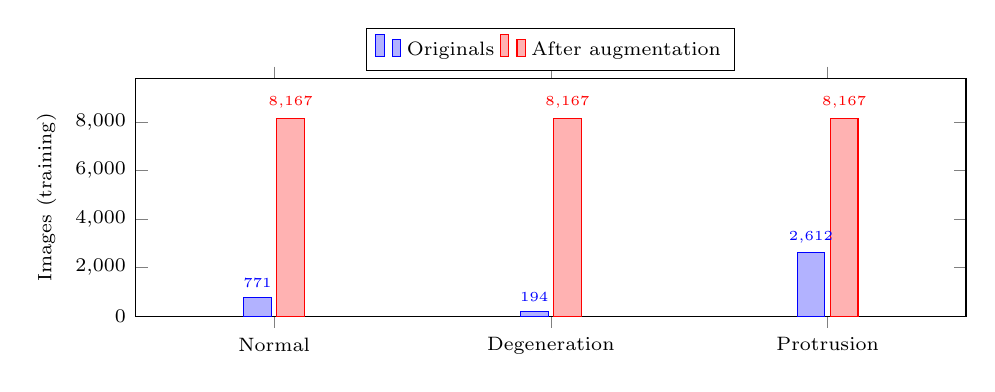
\begin{tikzpicture}
\begin{axis}[
  ybar, bar width=10pt, width=\columnwidth, height=4.6cm,
  symbolic x coords={Normal,Degeneration,Protrusion}, xtick=data,
  ymin=0, ymax=9800, ylabel={Images (training)},
  enlarge x limits=0.25, legend style={at={(0.5,1.03)},anchor=south,legend columns=2,font=\scriptsize},
  nodes near coords, every node near coord/.append style={font=\tiny},
  tick label style={font=\scriptsize}, ylabel style={font=\scriptsize}]
\addplot coordinates {(Normal,771) (Degeneration,194) (Protrusion,2612)};
\addplot coordinates {(Normal,8167) (Degeneration,8167) (Protrusion,8167)};
\legend{Originals, After augmentation}
\end{axis}
\end{tikzpicture}
\caption{Count-based balance in training: original ROIs and total after augmentation.}
\label{fig:balancechart}
\end{figure}

\subsubsection{Traceability}
Each file is named \arch{T2_TSE_SAG__0188_008_L4-L5__orig.png} (original) or \arch{..._aug012.png} (copy), with patient, slice and level. The manifest \arch{manifest_35k.csv} records, for each of the 35,007 images, its partition, class, patient, level, original ROI, reviewer and, for copies, the exact parameters (seed, angle, zoom, shifts, contrast and brightness); \arch{split_pacientes.csv} stores each patient's partition. The images are not uploaded to the repository: they are distributed as a 405~MB archive, and the repository keeps the manifests and the scripts that reproduce them from the public data.

\subsubsection{Checks}
The script verifies that (i) the patient sets of the three partitions are disjoint, (ii) every copy is in the same partition as its original, (iii) file names are unique, (iv) every PNG is intact, and (v) the total exceeds 35,000. The copies respect the declared ranges (angle between $-8^{\circ}$ and $8^{\circ}$, zoom and contrast between 0.90 and 1.10).

% ---------------------------------------------------------------------
\subsection{Class Balance and Level Bias}
\label{sec:balance}
The 1/3 balance per class is \emph{by count}, not by originals. Among the 5,123 original ROIs, Protrusion accounts for 73.0\% (3,738), Normal for 21.6\% (1,105) and Degeneration for 5.5\% (280); a classifier that always predicted Protrusion would be right about 73\% of the time. Copies equalize each class's contribution to training, but they add no new anatomy: the effective dataset size is the number of patients (399), and Degeneration, repeated about 42 times, has only 42 originals in the test partition, which leaves a wide margin of error on its recall. So that metrics are not inflated by near-identical copies, the main results are computed on the \textbf{originals} of the test partition, and the full set is reported separately. In addition, a model trained with a uniform prior tends to over-predict rare classes in the real population.

Table~\ref{tab:level} shows a strong bias: almost all pathology is concentrated at L4-L5 and L5-S1. A classifier that merely guessed the most frequent class at each level would get 3,842 of 5,123 ROIs right (75.0\%), so the level could act as a shortcut; shortcut learning makes measured performance overestimate real performance \cite{onglt2024}. Results are therefore also reported per level. This puts any accuracy threshold into perspective: a 95\% measured on these labels measures agreement with student labels and may be reached partly through the shortcut, and high internal figures tend to drop on external data \cite{yi2023}. For this reason, accuracy is accompanied by macro F1 and per-class recall: with imbalanced classes, the usual metrics are dominated by the majority class \cite{mosquera2024}.

\begin{table}[!htb]
\centering\footnotesize
\setlength{\tabcolsep}{4pt}
\caption{Eligible original ROIs by level and class}
\label{tab:level}
\begin{tabular}{lrrrrr}
\toprule
Level & Normal & Degen. & Protr. & Total & \% Protr. \\
\midrule
L1-L2 & 505 & 121 & 401   & 1,027 & 39.0 \\
L2-L3 & 383 & 94  & 550   & 1,027 & 53.6 \\
L3-L4 & 172 & 44  & 811   & 1,027 & 79.0 \\
L4-L5 & 15  & 5   & 1,005 & 1,025 & 98.0 \\
L5-S1 & 30  & 16  & 971   & 1,017 & 95.5 \\
\bottomrule
\end{tabular}
\end{table}

% III. Methodology (continued): formulation, models and evaluation protocol
% Subsections H to J. Based on the model selection section of Milestone 2
% and on docs/resultados/ (metadata.json of each model).

% ---------------------------------------------------------------------
\subsection{Problem Formulation and Metrics}
\label{sec:formulation}
The task is supervised multiclass classification: given the ROI $x$ of a disc, the model predicts a class $\hat{y}\in\{\text{Degeneration},\ \text{Normal},\ \text{Protrusion}\}$. The classes are nominal: the priority used during labeling (Section~\ref{sec:annotation}) is not a severity order, so the task was not posed as regression or ordinal classification.

The metrics are accuracy, per-class precision, recall and F1 and their macro averages, balanced accuracy (equal to macro recall), macro one-versus-rest area under the ROC curve, and log loss. Accuracy alone is misleading under this imbalance: a classifier that always predicted Protrusion would get 73\% of the original test ROIs right. The main comparison criterion is therefore macro F1, together with per-class recall \cite{mosquera2024}. To answer Q3, the clinical false-negative rate is also reported: the fraction of pathological discs (Degeneration or Protrusion) that the model classifies as Normal.

% ---------------------------------------------------------------------
\subsection{Models and Training}
\label{sec:models}
Four models were chosen that meet four criteria: (i) they can classify an ROI into three classes; (ii) they have precedents in lumbar MRI or in comparable medical tasks; (iii) they represent different families, so that the comparison is meaningful; and (iv) they can be trained with the same patient-level split and evaluated with the same metrics. All of them start from ImageNet-pretrained weights. The 128$\times$128~px grayscale ROIs are converted to three channels, resized to 224$\times$224~px and scaled to $[0,1]$; for ResNet-50 they are also normalized with the ImageNet mean and standard deviation. Table~\ref{tab:hyper} summarizes each model's configuration.

\begin{table*}[t]
\centering\footnotesize
\caption{Configuration of the four models. Values chosen among several options were set by validation macro F1 (or accuracy, for YOLO)}
\label{tab:hyper}
\begin{tabular}{>{\raggedright\arraybackslash}p{0.15\textwidth}>{\raggedright\arraybackslash}p{0.2\textwidth}>{\raggedright\arraybackslash}p{0.19\textwidth}>{\raggedright\arraybackslash}p{0.36\textwidth}}
\toprule
Model & Input & Optimization and loss & Hyperparameters \\
\midrule
1. YOLOv8s-cls & 224$\times$224 image & AdamW; cross-entropy & Initial rate $5\times10^{-4}$, final $\times 0.1$, cosine with 1 warm-up epoch; weight decay 0.01; 4 frozen layers; dropout 0.3; batch 64; up to 15 epochs, patience 4 \\
2. ResNet-50 & 224$\times$224 image, ImageNet normalization & AdamW; cross-entropy with 0.1 label smoothing & Rate $10^{-4}$ with cosine decay; weight decay 0.01; dropout 0.3; batch 64; up to 10 epochs, patience 4; best epoch: 2 \\
3. SVM & 2,048 features from the fine-tuned ResNet-50 $\to$ PCA 256 & Hinge loss (SVC) & RBF kernel, $\gamma$ = \texttt{scale}, one-versus-rest; $C\in\{0.1, 0.5, 2, 8\}$, chosen $C=0.1$ \\
4. Random Forest & Same as the SVM & Gini impurity & 300 trees; maximum depth $\in\{10, 20, \text{none}\}$, chosen 20 \\
\bottomrule
\end{tabular}
\end{table*}

\subsubsection{YOLOv8s-cls}
It is the classification variant of the YOLO family, the most common in the reviewed literature \cite{liawrungrueang2023,prisilla2023,wang2025}, and it is consistent with the rest of the pipeline, which already uses YOLO to detect the discs. It was fine-tuned with AdamW, cross-entropy, the first four layers frozen and a dropout of 0.3. Since the main augmentation is already in the files, online augmentation was limited to varying the crop aspect ratio (from 3:4 to 4:3) and brightness ($\pm 5\%$), without flips.

\subsubsection{ResNet-50}
It is a convolutional network from a different (residual) family, with precedents in lumbar disc classification \cite{tan2024,alkubaisi2022}. The first convolution and the first residual block were frozen, and the final layer was replaced by a dropout of 0.3 and a linear layer with three outputs. It was trained with AdamW, a cosine-decaying learning rate, cross-entropy with label smoothing of 0.1 and mild online augmentation (rotation of $\pm 6^{\circ}$, 4\% shift, zoom from 0.95 to 1.05, and brightness and contrast of $\pm 10\%$). The best epoch was chosen by validation macro F1, with early stopping.

\subsubsection{SVM and Random Forest on Deep Features}
A classical classifier on raw pixels treats each value separately and does not recognize shape. ResNet-50 was therefore used as a feature extractor: without its final layer, it yields 2,048 values per image, which are standardized, reduced to 256 components with principal component analysis (PCA; 80.0\% of the variance) and classified with an RBF-kernel SVM or a 300-tree Random Forest. The technique has precedents on this same corpus \cite{sari2025} and in other medical tasks \cite{khoiwal2024}; the Random Forest only has precedents on tabular data \cite{zhang2023} and is presented as our own extension. The scaler, the PCA and the classifiers are fitted on the training set only.

The initial design used ResNet-50 with frozen ImageNet weights, so that the SVM and the Random Forest would not depend on the fine-tuned network. On validation they performed poorly (macro F1 of 0.64 and 0.60), so the already fine-tuned ResNet-50 was adopted as the extractor (F1 of 0.80 and 0.79). The cost is that models 3 and 4 depend on model 2. The ImageNet version is kept as an ablation (Section~\ref{sec:res_q2}). As course baselines, a logistic regression and a KNN were also trained on the same features; they are not among the four models.

% ---------------------------------------------------------------------
\subsection{Evaluation Protocol}
\label{sec:protocol}
The four models use the same patient-level split (Table~\ref{tab:split}) and the same seed (42). Epochs, hyperparameters and variants were chosen on validation; the test set was evaluated once, with the final configuration. The variants tried on validation (other seeds, learning rates, smoothing and ensembles) are recorded in the repository.

The course guidelines recommend augmenting only the training set. Here, the validation and test sets were also augmented, to obtain the same count per class (Section~\ref{sec:augmentation}). Validation and test copies never enter training, so there is no leakage; even so, to keep near-identical copies from inflating the metrics, \textbf{the main results are computed on the 768 original test ROIs}, with the natural class proportions (42 Degeneration, 164 Normal and 562 Protrusion). The full, balanced test set with copies (5,253 images) is reported separately. With 768 images, the 95\% confidence interval of accuracy is about $\pm 2.2$ points (Wilson interval).


\section{Results and Discussion}
\label{sec:results}
% IV. Results and Discussion
% Figures: docs/resultados/comparacion/*.csv and confusion_test_orig.csv matrices
Unless otherwise stated, figures refer to the 768 original ROIs of the test partition (60 patients), evaluated once.

% ---------------------------------------------------------------------
\subsection{Class Distribution and Visual Differences (Q1)}
\label{sec:res_q1}
After human review, Protrusion accounts for 73.0\% of the 5,123 original ROIs, Normal for 21.6\% and Degeneration for 5.5\% (Section~\ref{sec:balance}). The distribution depends strongly on the level: Protrusion goes from 39.0\% at L1-L2 to 98.0\% at L4-L5 (Table~\ref{tab:level}). Degeneration, by contrast, appears mostly at L1-L2 and L2-L3, partly because at the lower levels a degenerated disc that also protrudes receives the Protrusion label.

The visual differences that guided labeling are those of the Pfirrmann scale and the consensus nomenclature \cite{pfirrmann2001,fardon2014}. A Normal disc has a bright nucleus on T2, clearly distinguishable from the annulus, and preserved height. In Degeneration the disc darkens due to loss of hydration and loses height, without disc material extending beyond the vertebral margin. In Protrusion the disc material extends beyond that margin, almost always towards the canal (Fig.~\ref{fig:rois}). Brightness thus distinguishes Normal from Degeneration, and the shape of the posterior contour identifies Protrusion. The distinction between bulge and herniation depends on the extent around the disc circumference, which is not visible on a sagittal slice, so these two classes were merged. Both pathologies also frequently co-occur: a degenerated disc may protrude, in which case it is labeled Protrusion under the priority rule, which anticipates the confusion between the two classes.

% ---------------------------------------------------------------------
\subsection{Comparison of the Four Models}
\label{sec:res_comparison}
Table~\ref{tab:results} summarizes the metrics. ResNet-50 achieved the highest accuracy (88.9\%, 683 of 768; 95\% CI: 86.5--91.0) and the highest macro F1 (0.769), followed by the SVM and the Random Forest (88.4\%) and YOLOv8s-cls (87.8\%). The confidence intervals of the four models overlap: the accuracy differences (one point at most) are not conclusive. The Random Forest obtained the highest ROC-AUC (0.942) and the lowest log loss (0.327), that is, the best-ranked and best-calibrated probabilities, although its macro F1 is the lowest of the four. The ensemble of the four models does not improve on ResNet-50 in accuracy or F1.

\begin{table*}[t]
\centering\footnotesize
\setlength{\tabcolsep}{4.5pt}
\caption{Results on the test partition. The ``originals'' columns use the 768 original ROIs; metrics are macro averages. ``Train'' is accuracy on the original training ROIs and ``Full test'' is the balanced set with copies (5,253 images). Best of the four models in bold}
\label{tab:results}
\begin{tabular}{lrrrrrrrrr}
\toprule
 & \multicolumn{6}{c}{Test, originals (768)} & & \multicolumn{2}{c}{Full test} \\
\cmidrule(lr){2-7}\cmidrule(lr){9-10}
Model & Accuracy & Precision & Recall & F1 & ROC-AUC & Log loss & Train & Accuracy & F1 \\
\midrule
1. YOLOv8s-cls        & 0.878 & 0.771 & 0.732 & 0.750 & 0.931 & 0.488 & 0.984 & 0.759 & 0.752 \\
2. ResNet-50          & \textbf{0.889} & 0.795 & \textbf{0.751} & \textbf{0.769} & 0.919 & 0.329 & 0.971 & \textbf{0.775} & \textbf{0.768} \\
3. SVM (RBF)          & 0.884 & 0.797 & 0.718 & 0.748 & 0.899 & -- & 0.979 & 0.754 & 0.746 \\
4. Random Forest      & 0.884 & \textbf{0.810} & 0.710 & 0.746 & \textbf{0.942} & \textbf{0.327} & 0.998 & 0.743 & 0.731 \\
\midrule
\multicolumn{10}{l}{\emph{Additional comparisons}} \\
Ensemble of the 4 (average)          & 0.889 & 0.782 & 0.721 & 0.745 & 0.947 & 0.321 & 0.989 & 0.762 & 0.752 \\
Logistic regression (baseline)       & 0.878 & 0.819 & 0.696 & 0.740 & 0.896 & 0.732 & 0.988 & 0.730 & 0.717 \\
KNN (baseline)                       & 0.888 & 0.794 & 0.722 & 0.751 & 0.858 & 1.000 & 0.980 & 0.758 & 0.749 \\
SVM, ImageNet features               & 0.776 & 0.563 & 0.600 & 0.576 & 0.829 & -- & 0.841 & 0.633 & 0.619 \\
Random Forest, ImageNet features     & 0.753 & 0.518 & 0.546 & 0.524 & 0.831 & 0.726 & 0.999 & 0.598 & 0.577 \\
\bottomrule
\multicolumn{10}{l}{\scriptsize The SVM does not output probabilities, so it has no log loss.}
\end{tabular}
\end{table*}

On the full, balanced test set, accuracy drops to 74--78\%. That set weights the three classes equally, so Degeneration, the hardest class, counts as much as Protrusion. The gap between the two figures shows how much of the accuracy on originals comes from the majority class.

% ---------------------------------------------------------------------
\subsection{Per-Class Results and False Negatives (Q3)}
\label{sec:res_q3}
Table~\ref{tab:perclass} and Fig.~\ref{fig:confusion} show per-class behavior. The four models recognize Protrusion with a recall of 0.94 to 0.95 and the Normal class with 0.76 to 0.81. Degeneration is the weak class: ResNet-50 and YOLOv8s-cls detect half of the 42 cases (95\% CI: 0.36--0.64), and the SVM and the Random Forest between 40 and 43\%. Their errors go mainly towards Protrusion (12 to 17 cases depending on the model), consistent with the co-occurrence of both pathologies described in Section~\ref{sec:res_q1}. The second most frequent confusion is Normal predicted as Protrusion (26 to 36 cases).

\begin{figure*}[t]
\centering
\includegraphics[width=0.95\textwidth]{confusion_matrices_en.png}
\caption{Confusion matrices of the four models on the 768 original test ROIs. Each cell shows the number of cases and the percentage of its row (true class).}
\label{fig:confusion}
\end{figure*}

If Degeneration and Protrusion are grouped as ``pathological'', the four models classify between 5.0 and 5.5\% of the 604 pathological discs as Normal; that is, their sensitivity for detecting pathology is 94.5 to 95.0\%. In clinical false negatives, the SVM and the Random Forest are slightly better (30 cases versus 32 and 33), but at the cost of lower recall on Degeneration. No model dominates on every metric.

\begin{table}[!htb]
\centering\footnotesize
\setlength{\tabcolsep}{3pt}
\caption{Per-class recall and F1 on the original test ROIs, and fraction of pathological discs (604) classified as Normal (FN)}
\label{tab:perclass}
\begin{tabular}{lrrrrrrr}
\toprule
 & \multicolumn{3}{c}{Recall} & \multicolumn{3}{c}{F1} & \\
\cmidrule(lr){2-4}\cmidrule(lr){5-7}
Model & Degen. & Normal & Protr. & Degen. & Normal & Protr. & FN \\
\midrule
YOLOv8s-cls   & 0.500 & 0.756 & 0.941 & 0.545 & 0.775 & 0.929 & 5.3\% \\
ResNet-50     & 0.500 & 0.811 & 0.941 & 0.568 & 0.806 & 0.935 & 5.5\% \\
SVM           & 0.429 & 0.774 & 0.950 & 0.522 & 0.791 & 0.932 & 5.0\% \\
Random Forest & 0.405 & 0.774 & 0.952 & 0.515 & 0.791 & 0.931 & 5.0\% \\
\bottomrule
\end{tabular}
\end{table}

Regarding Q3, ResNet-50 is the architecture with the best accuracy and macro F1, but none reaches the 90\% target: ResNet-50 falls 1.1 points short, within its confidence interval but below the target. On validation, all variants tried (two architectures, three seeds, regularization and ensembles of up to eight networks) plateaued between 86 and 87.5\% on the originals. That such different methods hit the same ceiling suggests that the limit lies in the data rather than in the model.

% ---------------------------------------------------------------------
\subsection{Classical Classifiers versus Deep Networks (Q2)}
\label{sec:res_q2}
On features from the fine-tuned ResNet-50, the SVM and the Random Forest match the networks (88.4\% accuracy and macro F1 of 0.748 and 0.746), and so do the logistic regression and the KNN (Table~\ref{tab:results}). With non-fine-tuned ImageNet features, however, they drop to 77.6 and 75.3\% accuracy and to a macro F1 of 0.576 and 0.524, and Degeneration almost disappears (recall of 0.21 and 0.10). The answer to Q2 is therefore nuanced: a classical classifier can be as reliable as a deep network, but only if it operates on features already learned by a network fine-tuned to the task. In that case, what separates the classes lies in the representation, not in the final classifier. Hand-crafted features (mean disc intensity, height or contour) were not tested and are left for future work.

% ---------------------------------------------------------------------
\subsection{Overfitting}
\label{sec:res_overfitting}
The four models get between 97.1 and 99.8\% of the original training ROIs right, versus 87.8--88.9\% on the test set (Table~\ref{tab:results}). The networks reach their best validation epoch very early (ResNet-50 at epoch 2), after which training error keeps decreasing without improving validation. The Random Forest is the extreme case (99.8\% on training). The regularization measures (frozen layers, dropout, weight decay, label smoothing, online augmentation and early stopping) contained overfitting without eliminating it. This is expected with 279 training patients and 194 Degeneration originals each repeated about 42 times.

% ---------------------------------------------------------------------
\subsection{Vertebral-Level Bias}
\label{sec:res_level}
Table~\ref{tab:levelres} compares ResNet-50 accuracy at each level with that of a trivial classifier that always predicts the most frequent class of that level in the test set. The trivial classifier gets 74.7\% of the total right, very close to the 73\% of always predicting Protrusion. At L4-L5 and L5-S1, where almost everything is Protrusion, ResNet-50 barely beats the trivial classifier (97.4 versus 94.8\% and 94.2 versus 94.2\%). Its real advantage lies at L1-L2 and L2-L3, where the classes are more evenly spread (30 points at L1-L2 and 29 at L2-L3). Thus, part of the overall accuracy may come from the level rather than from the image, as in shortcut learning \cite{onglt2024}; the lower levels, where the shortcut is easiest, weigh as much in the overall accuracy as the upper ones.

\begin{table}[!htb]
\centering\footnotesize
\caption{Per-level accuracy of ResNet-50 versus a classifier that predicts the most frequent class of each level (original test ROIs)}
\label{tab:levelres}
\begin{tabular}{lrrr}
\toprule
Level & ROIs & Most frequent class & ResNet-50 \\
\midrule
L1-L2 & 153 & 48.4\% & 78.4\% \\
L2-L3 & 153 & 56.2\% & 85.6\% \\
L3-L4 & 154 & 79.9\% & 89.0\% \\
L4-L5 & 154 & 94.8\% & 97.4\% \\
L5-S1 & 154 & 94.2\% & 94.2\% \\
\midrule
Total & 768 & 74.7\% & 88.9\% \\
\bottomrule
\end{tabular}
\end{table}

% ---------------------------------------------------------------------
\subsection{Comparison with the State of the Art}
\label{sec:res_sota}
The figures in this work are lower than those in the literature (97--99\%) \cite{sari2025,liawrungrueang2023}, but they are not directly comparable. Sar{\i} and Atasoy used the same corpus, but on a binary task, with T1 slices and cross-validation without a declared patient-level split \cite{sari2025}; here the task has three highly imbalanced classes, the split is patient-level and evaluation is done on originals the model never saw. Natalia \emph{et al.}, on the same corpus and predicting the Pfirrmann grade, reported a mean accuracy of 88.1\% \cite{natalia2024}, of the same order as the one obtained here. In addition, high internal figures tend to drop under external validation \cite{yi2023,nigru2024}, which this work could not perform. Finally, the labels come from students without a radiologist, so accuracy measures agreement with those labels and not with a clinical diagnosis \cite{shi2024}.


\section{Conclusions}
\label{sec:conclusions}
% V. Conclusions
Starting from a public corpus of 515 patients, this work built a traceable dataset of 5,123 lumbar disc ROIs from 399 patients in three classes and compared four models on it under the same patient-level split and the same metrics. The answers to the research questions are as follows.

\textbf{Q1.} The dataset is highly imbalanced: Protrusion accounts for 73.0\% of the ROIs, Normal for 21.6\% and Degeneration for 5.5\%, and pathology concentrates at L4-L5 and L5-S1. The disc's T2 signal separates Normal from Degeneration, and the shape of the posterior contour identifies Protrusion; Herniation and Bulge cannot be separated on the sagittal plane, which forced their merge.

\textbf{Q2.} The SVM and the Random Forest match the networks (88.4\% accuracy) only when they use features from a ResNet-50 fine-tuned to the task; with generic ImageNet features they drop to 75--78\% and barely detect Degeneration. They are faster to fit, but they do not replace the network: they depend on it.

\textbf{Q3.} ResNet-50 obtained the highest accuracy (88.9\%) and the highest macro F1 (0.769), with no conclusive differences from the other three models and without reaching the 90\% target. All four classify only 5.0 to 5.5\% of pathological discs as Normal, but detect just 40 to 50\% of Degeneration cases. Part of the accuracy is explained by the vertebral level.

Overall, the limiting factor was not the architecture but the data: few original Degeneration images, student labels without a radiologist and a strong level bias. This is why per-class and per-level metrics matter as much as overall accuracy.


\subsection{Limitations and Future Work}
% Limitations and future work. Goes inside "V. Conclusions".
The main limitations are the following:
\begin{itemize}
  \item Labels come from students, without a radiologist, reviewed while seeing a model's suggestion, and inter-annotator agreement was not measured (Section~\ref{sec:annotation}).
  \item Only the sagittal plane is available; Herniation and Bulge cannot be separated and were merged after seeing the data.
  \item A single 1.5~T MRI scanner, with no scanner diversity and no external validation, which the literature recommends for these models \cite{nigru2024,wang2025}.
  \item The effective size is 399 patients; copies add no new anatomy. Degeneration has few patients (81, 17 and 22 in the three partitions) and only 42 originals in the test set, which leaves a wide margin of error on its recall.
  \item Level bias and uniform prior (Sections~\ref{sec:balance} and \ref{sec:res_level}).
  \item The public dataset does not include a patient identifier: the \texttt{PatientID} field is empty in all the original \texttt{.IMA} files, which depends entirely on the source and not on this work. The folder number was therefore used as the patient identifier, following the source's organization (one folder per patient, 515 in total), and the patient-level split was done by folder. Among the 414 folders used, no \texttt{StudyInstanceUID} or \texttt{StudyTime} is repeated, so there is no sign of duplicates; only if the source itself had spread one person across two folders could there be an overlap between partitions, and this cannot be verified without the original identifier.
  \item A slice selection error lost 36 patients and left another 8 with a parasagittal slice (Section~\ref{sec:cleaning}).
  \item The detector metrics come from a training re-run and not from the model that generated the ROIs.
  \item The SVM and the Random Forest depend on the fine-tuned ResNet-50, so they are not independent models, and each official model corresponds to a single seed.
  \item The system is an academic tool, not a diagnostic one.
\end{itemize}

As future work, the Degeneration labels could be checked against the radiologist-validated Pfirrmann grades available for this same corpus at L3-L4, L4-L5 and L5-S1 \cite{masood2026}, and the models could be evaluated on multicenter, expert-annotated datasets \cite{richards2026}. Fixing the slice filtering, by selecting only the T2 TSE series, would also recover the 36 lost patients. Since Degeneration and Protrusion co-occur in the same disc, a multi-label formulation, instead of the priority rule, could reduce the confusion between them. Finally, adding axial slices would make it possible to separate Herniation and Bulge again, and hand-crafted features (disc intensity and height) would complete the answer to Q2.


\section*{Acknowledgment}
The authors thank S. Sudirman and co-authors for releasing, in open access, the dataset that made this work possible \cite{sudirman2019}.

\bibliographystyle{IEEEtran}
\bibliography{references}

\end{document}
